\documentclass{article}
\usepackage{amsmath, graphicx}
\graphicspath{  {./images/}  }

\title{Ch. 6 HW/CW}
\author{Principles of Microeconomics}
\date{\today}

\begin{document}

\maketitle

\begin{enumerate}

\item The tax burden falls entirely on the team owners because their supply of seats is perfectly inelastic. When demand shifts down, the price that consumers pay doesn't move at all, and the price that producers receive goes down by \$5, the full amount of the tax.
	\begin{center}
	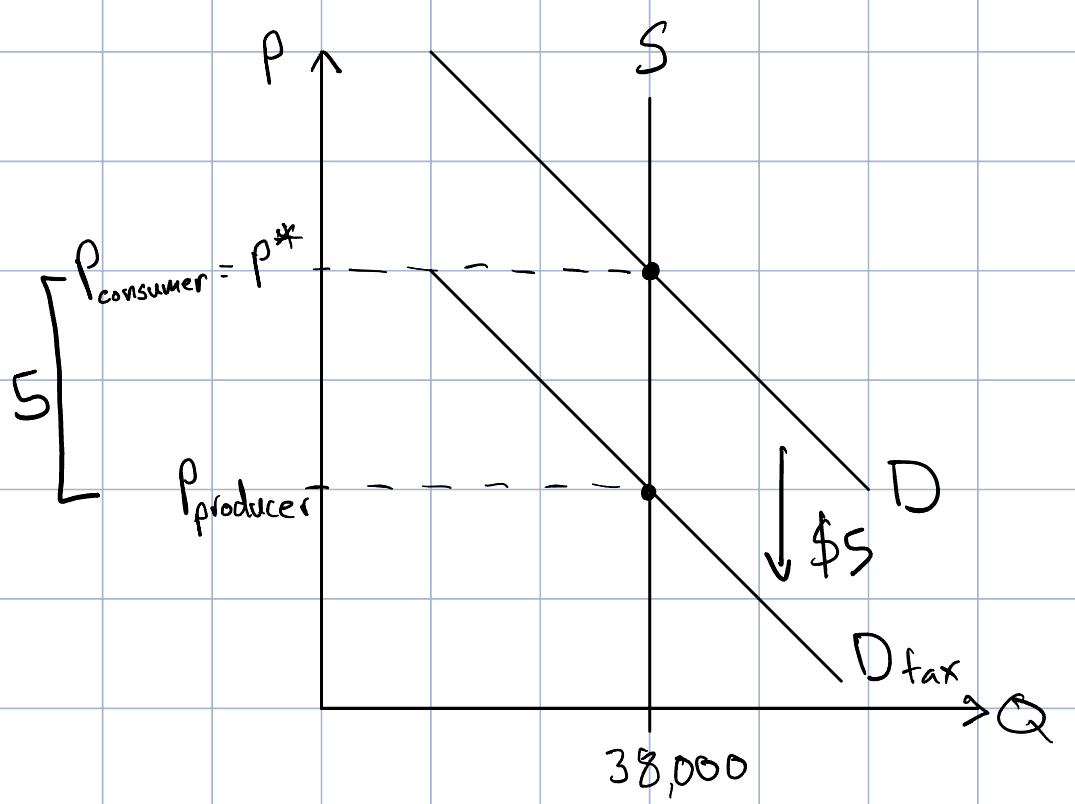
\includegraphics[width = 0.5\textwidth]{problem1}
	\end{center}
	
\newpage
	
\item
	\begin{enumerate}
	
	\item
		\begin{align*}
		Q_S &= Q_D \\
		2P^* &= 300 - P^* \\
		3P^* &= 300 \\
		P^* &= 100 \\
		Q^* &= 2P^* = 2(100) = 200 
		\end{align*}
		
	\item A shortage develops because the price ceiling is binding. Therefore, $P = P_{ceiling} = 90$. 
		\begin{align*}
		Q_S &= 2P_{ceiling} = 2(90) = 180 \\
		Q_D &= 300 - P_{ceiling} = 300 - 90 = 210 \\
		Shortage &= Q_D - Q_S = 210 - 180 = 30
		\end{align*}
		
		\begin{center}
		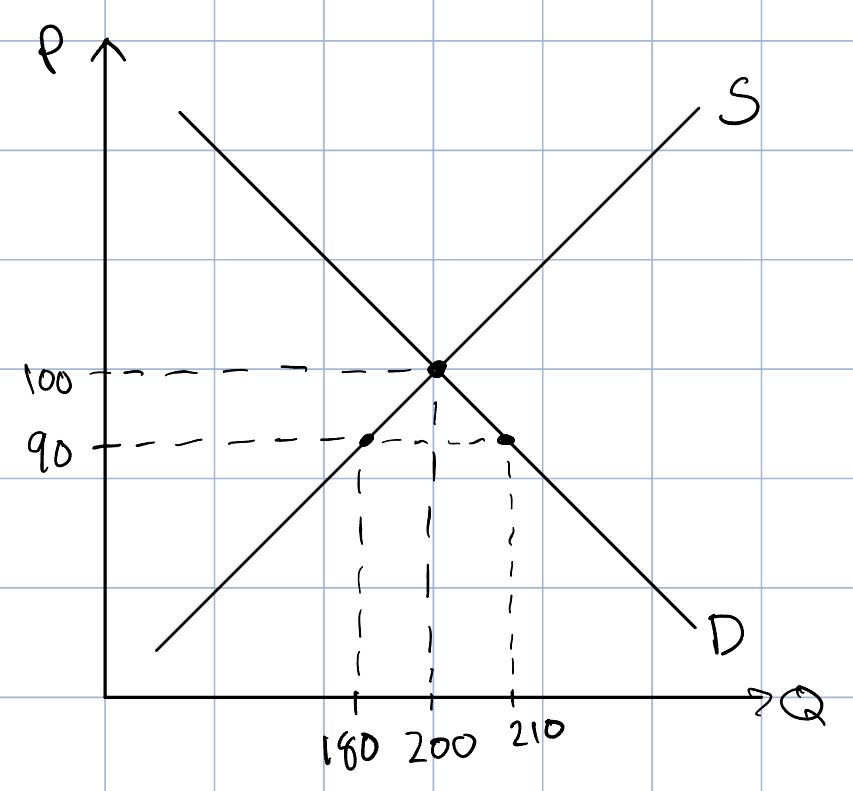
\includegraphics[width = 0.5\textwidth]{problem2b}
		\end{center}
		
	\item Neither develops because the price floor isn't binding. Therefore, $P = P^* = 100$, and $Q_S = Q_D = Q^* = 200$. 
	
	\newpage
	
	\item No shortage or surplus develops.
		\begin{align*}
		Q_D &= 300 - P_{consumer} \\
		Q_S &= 2(P_{consumer} - 30) = 2P_{consumer} - 60 \\
		300 - P_{consumer} &= 2P_{consumer} - 60 \\
		360 &= 3P_{consumer} \\
		120 &= P_{consumer} \\
		P_{producer} &= P_{consumer} - 30 = 120 - 30 = 90 \\
		Q_{tax} &= Q_S = Q_D = 300 - 120 = 180
		\end{align*}
		
		\begin{center}
		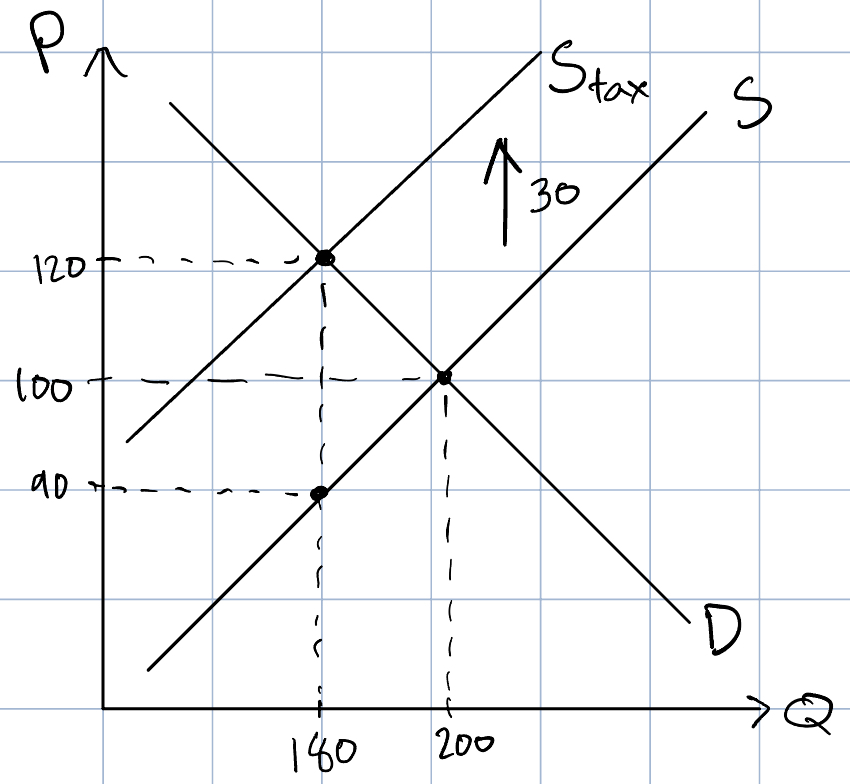
\includegraphics[width = 0.5\textwidth]{problem2d}
		\end{center}
	
	\end{enumerate}

\newpage

\item 
	\begin{align*}
	2,500 - 3P^* &= 5P^* - 100 \\
	2,600 &= 8P^* \\
	325 &= P^* \\
	Q^* &= 5(325) - 100 = 1,525 \\
	Q_{ceiling} &= 5P_{ceiling} - 100 = 5(300) - 100 = 1,400 \\
	\Delta Q &= Q^* - Q_{ceiling} = 1,525 - 1,400 = 125
	\end{align*}
	
	\begin{center}
	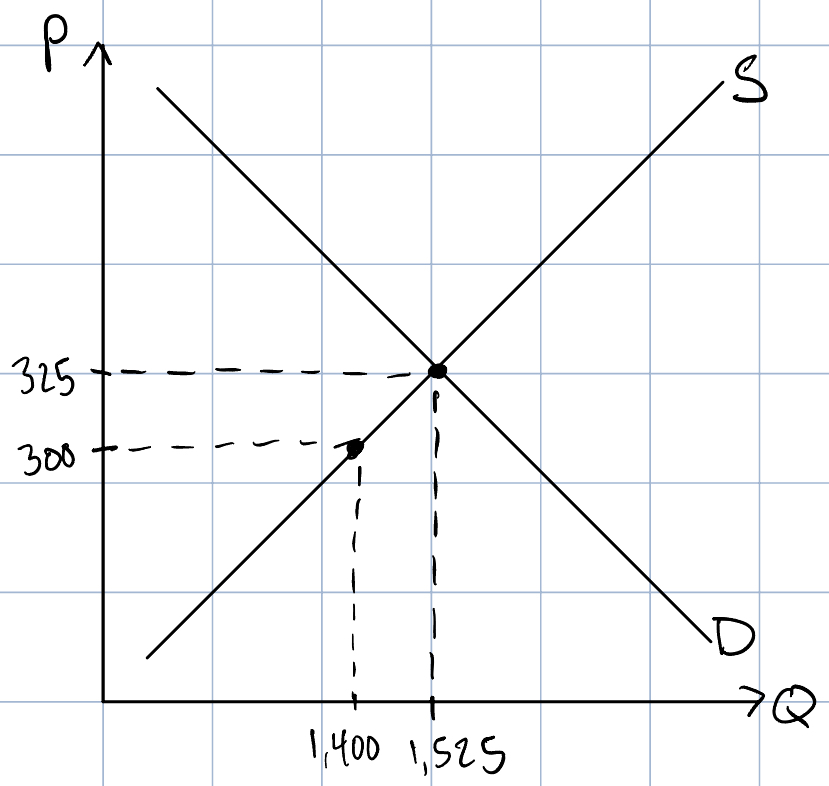
\includegraphics[width = 0.5\textwidth]{problem3}
	\end{center}
	
\newpage
	
\item
	\begin{enumerate}
	
	\item
		\begin{align*}
		Q_D &= Q_S \\
		150 - 5P^* &= 5P^* \\
		150 &= 10P^* \\
		15 &= P^* \\
		Q^* &= 5P^* = 5(15) =  75 \\
		Q_{floor} &= 150 - 5P_{floor} = 150 - 5(20) = 50 \\
		\Delta Q &= Q^* - Q_{floor} = 75 - 50 = 25
		\end{align*}
		
		\begin{center}
		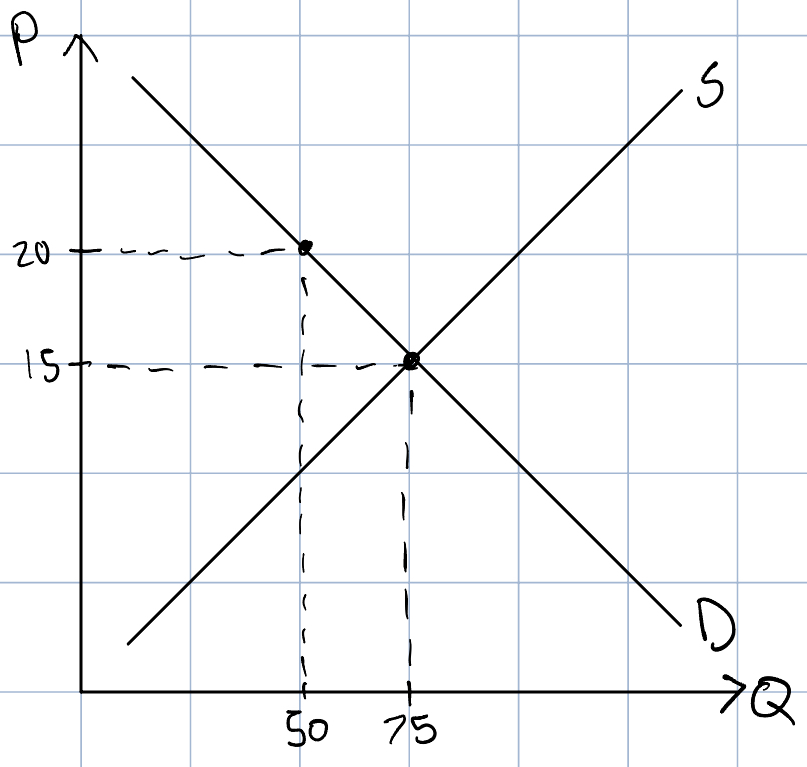
\includegraphics[width = 0.5\textwidth]{problem4a}
		\end{center}
		
	\newpage
	
	\item
		\begin{align*}
		Q_D &= 150 - 5P_{consumer} \\
		Q_S &= 5(P_{consumer} - 2)  = 5P_{consumer} - 10 \\
		150 - 5P_{consumer} &= 5P_{consumer} - 10 \\
		160 &= 10P_{consumer} \\
		16 &= P_{consumer} \\
		P_{producer} &= P_{consumer} - 2 = 16 - 2 = 14 \\
		Q_tax &= 150 - 5P_{consumer} = 150 - 5(16) = 70
		\Delta Q &= 75 - 70 = 5
		\end{align*}
		
		\begin{center}
		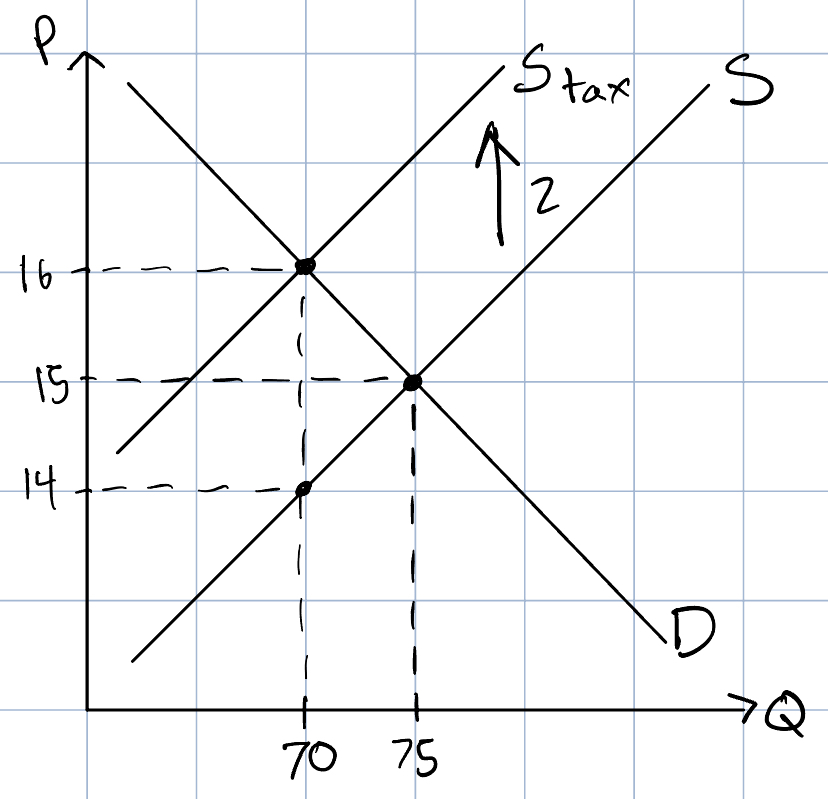
\includegraphics[width = 0.5\textwidth]{problem4b}
		\end{center}
		
	\item Consumer: $\frac{|P_{consumer} - P^*|}{t} \cdot 100 = \frac{16 - 15}{2} \cdot 100 = 50\%$ \\
		Producer: $\frac{|P_{producer} - P^*|}{t} \cdot 100 = \frac{|14 - 15|}{2} \cdot 100 = 50 \%$
	
	\end{enumerate}
	
\newpage
	
\item
	\begin{enumerate}
	
	\item
		\begin{align*}
		600 - 150P^* &= 200P^* - 100 \\
		700 &= 350P^* \\
		2 &= P^* \\
		Q^* &= 600 - 150(2) = 300
		\end{align*}
	
	\item
		\begin{align*}
		Q_S &= 200P_{producer} - 100 \\
		Q_D &= 600 - 150(P_{producer} + 0.875) = 468.75 - 150P_{producer} \\
		200P_{producer} - 100 &= 468.75 - 150P_{producer} \\
		350P_{producer} &= 568.75 \\
		P_{producer} &= 1.625 \\
		P_{consumer} &= P_{producer} + 0.875 = 1.625 + 0.875 = 2.50
		\end{align*}
		
		\begin{center}
		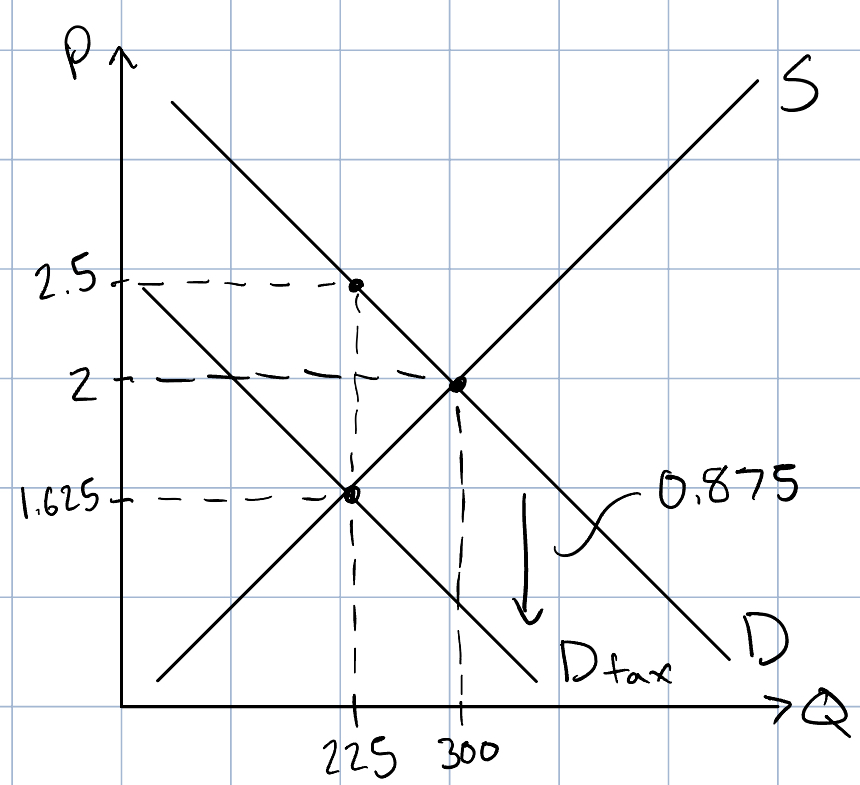
\includegraphics[width = 0.5\textwidth]{problem5b}
		\end{center}
		
	\item $Q_{tax} = 200P_{producer} - 100 = 200(1.625) - 100 = 225$
	
	\end{enumerate}

\end{enumerate}

\end{document}